\chapter{Twitter specific background}
\label{chapter:twitterbackground}

\section{The role of the graph store}
\label{section:api}
Twitter is a service where users can create a profile and post short messages, and can suscribe to other user's messages by `following' them.  The main Twitter objects are users, their  messages  (known as `tweets' in Twitter jargon), and their subscriptions to other users. Each of these objects has associated metadata such as user name, user profile information,  user location,  message timestamp, and timestamp of when one user followed another. 

is  a time ordered list of all tweets from users they follow, and it can be computed from the other lists by (conceptually) joining the tweets table with the follows table. (a follows b and b tweeted c, therefore a sees c in timeline.).  A user can choose follow any other user freely, (there is no hard limit), and a user can be followed by anyone who chooses to.  These objects are stored in different services, there is a user store, a tweet store, and the service in charge of the follows relation is what we call the graph store in this thesis. The source for the current implementation of the service, FlockDB, is publicly available at \hyperlink{https://github.com/twitter/flockdb}{github.com/twitter/flockdb}. 

At Twitter there are three main types of query operations expected of the graph store interface.  The only type of  update to the data base is to create, modify or delete a single edge given its endpoints.

The first basic query, {\code getEdge(v,w)} is the edge metadata lookup given the two endpoints of an edge. Metadata includes  timestamps for when the edge was created, when it was last updated and other edge properties such as the type of the edge. For example, it could be a standard `follow', or a `follow via sms', or a `blocked'.

Edges are directed, in Twitter `@A follows @B' does not imply `@B follows @A', but `@A follows @B' is a fact that may be queired via both @A and @B. So there need to be indexing on both endpoints. Also because of that, there is some degree of duplicaton. An update to one of the edges will need to be applied to two possibly separate locations.

At the application level, this query enables the website to inform a user visiting a profile whether she follows it. In the case of blocked users, the metadata also enables the system to hold their tweets from being delivered to the blocker.

The second query is, given a vertex A, return all its adjacent vertices: {\code getFanout(v)}. The real, complete, interface allows more specfic paramters, for instance, in a directed graph there are two directions to choose from so we could  wish to read  all vertices that follow A, or all vertices that A follows.  Another possible query is to read all non-blocked users, which involves a scan plus  some filtering out of blocked users. In general a fanout query can select users   for some property in the edge metadata.  There are other variations on this, we can ask for user given number of vertices. We can also use the query to retrieve  for example the latest one, or `mutual follows'

The interface also offers to page through the results of a query. This involves specifying a page size and an offset. Also, the ordering of the result set can be set to the order in which follows happened. This provides a way to answer queries for the most recent follower, or the 10 most recent followers.

Most importantly, the fanout operation enables tweet routing and delivery. Whenever user @A tweets, the effects of that action must be propagated to @B, and @C if they follow @A, and must be withheld from user @D if the edge specifies it is blocked. Or alternatively, whenver @B signs into the service, tweets from @A must be collected and shown in her timeline.  

There are many alternatives on how to make this process of delivery as efficient as possible, like in \ref{frenzy}. But either way, the routing table needs to be consulted for either pulling or pushing.  In fact,  a system such as \ref{frenzy} would require potentially more information to be stored in the routing table (the graph db).

The third query is the intersection of neighbors {\code getIntersection(v,w)}. Intersection requires a lot more work than fanout or edge, respectively. In fact, it implies at least two fanout type operations plus the added work to intersect the results. This work can be heavy, especially if the fanout sets are not sorted by id to start with.

  One option to implement this operation is to let  the server only implement fanouts, and have the clients intersect the results themselves. This approach reduces cpu work at the server,  but on the other hand, increases external bandwidth use for many results that eventually get filtered.   Like with fanouts, There are many variations on this query and they may be paginated or limited to ony the first few results as well.

There are many clear uses for this query, such as computing a similarity score between users etc (for example, cosine similarity), or we may want to intersect the followers of @A with the folowers of @B to see how much they have in common. We could also intersect the set of users followed by @A with the set of followers of @B, this gives us all the paths from @A to @B via the follows relation, but some of thse are not reaully used for website serving.  There are several real use cases for this operation, though. When a user @A visits a friend  @B's page, the website shows @A a limited set of common friends.  When a user @A visits a stranger @B's profile page, the website shows @A all of the people known by @A, which are already folllowing @B.  Finally, when a public conversation betweeen user @A and user @B occurs, the application  requires that only users following both @A and @B  receive these messages. So, like with fanouts, intersection queries are also needed for message routing.

The database also supports more complicated set operations, for example three way intersections, and differences.

\section{Notes on workload and data}

The information shown about the kinds of operatons, workloads, and the kind of data stored in the data base are relevant to designing the storage system.  For example,  areas such as the interface language (express set operations?), query processing(push operations to individual nodes?, check for wide differences in size for intersections, treat different users differently), data partitioning  across nodes (locate followers together?), and storage data structures (index for each view of a directed edge: from its source, or  from its destination). It also gives an idea of which things we do not need to support, such as queries about shortest paths, or computing page rank, 

\subsection{Workload}
\label{section:workload}
The graph store workload is made up of a mix of the queries in the section \ref{section:api}. One of the goals of of this project was to have a clearer picture of how they API was really used.  The broad questions were what kind of queries are more popular? are there heavily queried users? and whether  there is a relation between the the queries and the follows graph itself.  To answer these, we logged a sample of the requests into the current graph service and took about 300 million samples indicating the kind of operation and the arguments to it. The aggregate results are shown in table~\ref{table:workload}.

\newcommand{\other}{other fanouts, etc}

\begin{table}[h!]
\centering
\caption{Graph procedures usage table aggregated from a sample of query logs. Excludes counts, inserts. the \other category includes fanouts done at larger offsets and a few unrelated operations} 
\label{table:workload}
\begin{tabular}{l|c}
operation type & frequency \\
\hline
fanout (small page, zero offset) & 70\% \\
fanout (large page, zero offset) & 10\% \\
intersection & 1.5\% \\
edge metadata & 0.5\%\\
\other & 18\%\\
\end{tabular}
\end{table}

 The table shows small page fanouts are the most popular type of query,  that larger types of fanouts are the second most popular. Also, it reflects that there are two main clusters of page sizes used as arguments. Some are very small (the `small page' category, roughly less than 10 results) The rest are in the hundreds or thousands. Because a full logical fanout query can be split into several paged requests at different offsets, the `other fanouts' category may include counts of the same logical fanout for some large nodes.   The page size given to fanout bounds how expensive the operation can be. Requesting the latest 1 or 10 followers is lightweight, but requesting 1000 of them  involes a lot more more work. Intersections happen relatively seldom in this sample, suggesting they may not be as important.  Surprisingly, edge metadata queries seem to happen seldom.

On the other hand the importance of a particular query is a product of its frequency and on the load each places on the system. A single intersection implies at least 2 fanouts and at some sort-merging (or worse), so their effect on system load is larger than their frequency alone suggests. Since the light weight operations represent about 70\% of the requests, the heavyweight operations need to require about 5x more work than a light weight operatoin per request in order to be as significant in the total work load of the system. Finally, the logs excluded writes to edges.

A second important aspect is how uniform these queries are across users. By grouping a small subset of about 1000 different users tallying the number of operations they were involved in, we found the results of figure \ref{fig:queryfreq}.

\begin{figure}
\centering
\renewcommand{\gridscale}{3.5in}
 \subfigure{\includegraphics[width=\gridscale]{figures/edgeQs.png}}\\
 \subfigure{\includegraphics[width=\gridscale]{figures/fanoutQs.png}}\\
 \subfigure{\includegraphics[width=\gridscale]{figures/intersectionQs.png}}
\caption{log-log histograms of query frequency.}
\label{fig:queryfreq}
\end{figure}

All query histograms in Figure \ref{fig:queryfreq} show variation of orders of magnitude on how often a user gets queried. The plots also show that in the case of dge queries and intersection queries the overwhelming majority of users is involved in very few (in this scale any constant change in the plot implies an order of magnitude in reality). While the fanout queries don't seem to show a clear trend, the intersection query shows an almost linear shape of frequency decay. This is the expected shape for a power law and other fat tail distributions. The samples used for these plots are biased to include only users appearing in the logs with at least one intersection, so these plots aren't fully representative, but they do convey the high locality of the query workload.

Another useful datum is the degree of dependence between different kinds of queries. We already know some users are queried for fanouts much more often than others, but we maight also want to know whether this frequency correlates with how often they are arguments to intersection queries, or if edge queries involving them are occur more often too. The results of this experiment are shown in Figure~\ref{fig:querycorr}. One reason this is an important piece of information has to do with how work is spread. If some users are queried much more than others, then even after spreading users evenly across machines the work may not be spread evenly. On the other hand, this kind of bias also helps us. Having a lot of the queries go to a few of the users implies adaptive techniques like caching have a chance of being effective.

\begin{figure}
\centering
\renewcommand{\gridscale}{3.5in}
 \subfigure{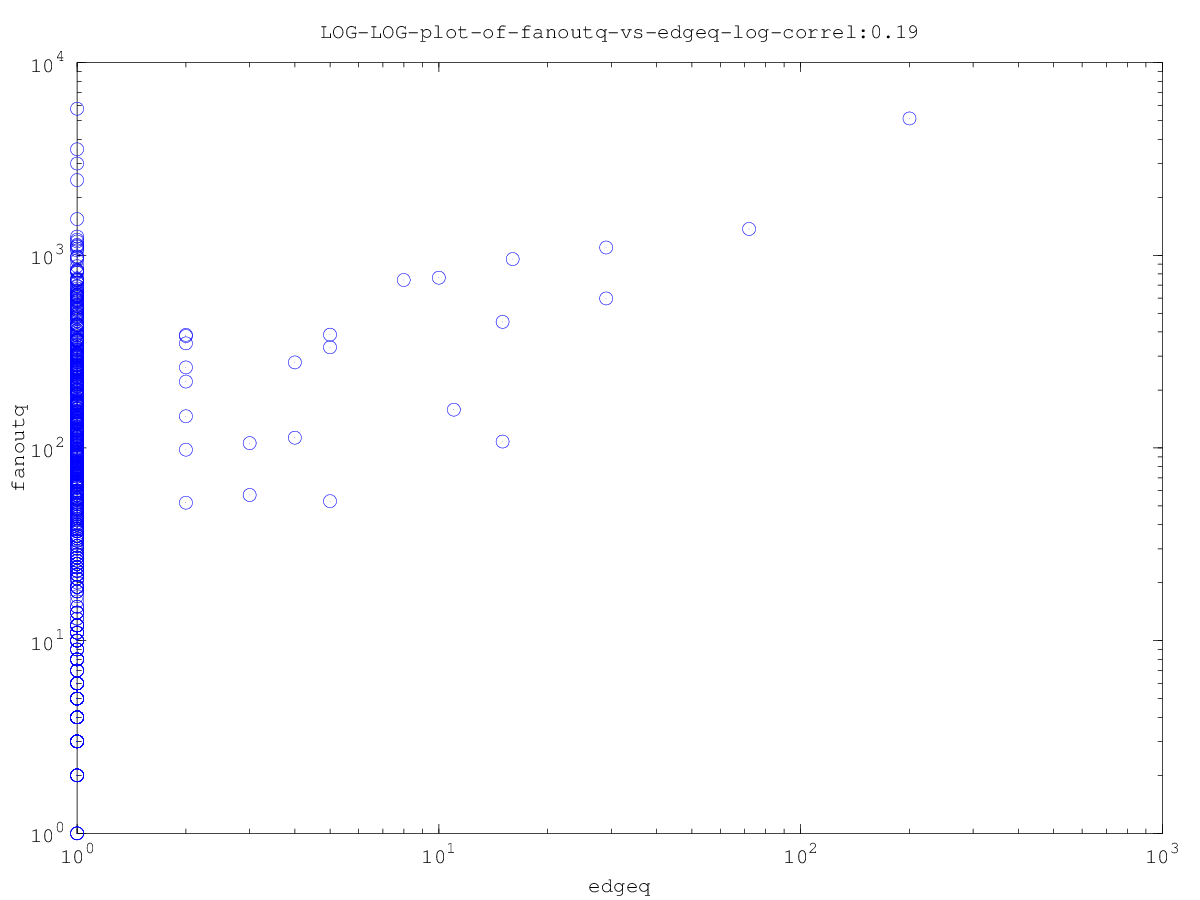
\includegraphics[width=\gridscale]{figures/LOG-LOG-plot-of-fanoutq-vs-edgeq-log-correl019.png}}\\
 \subfigure{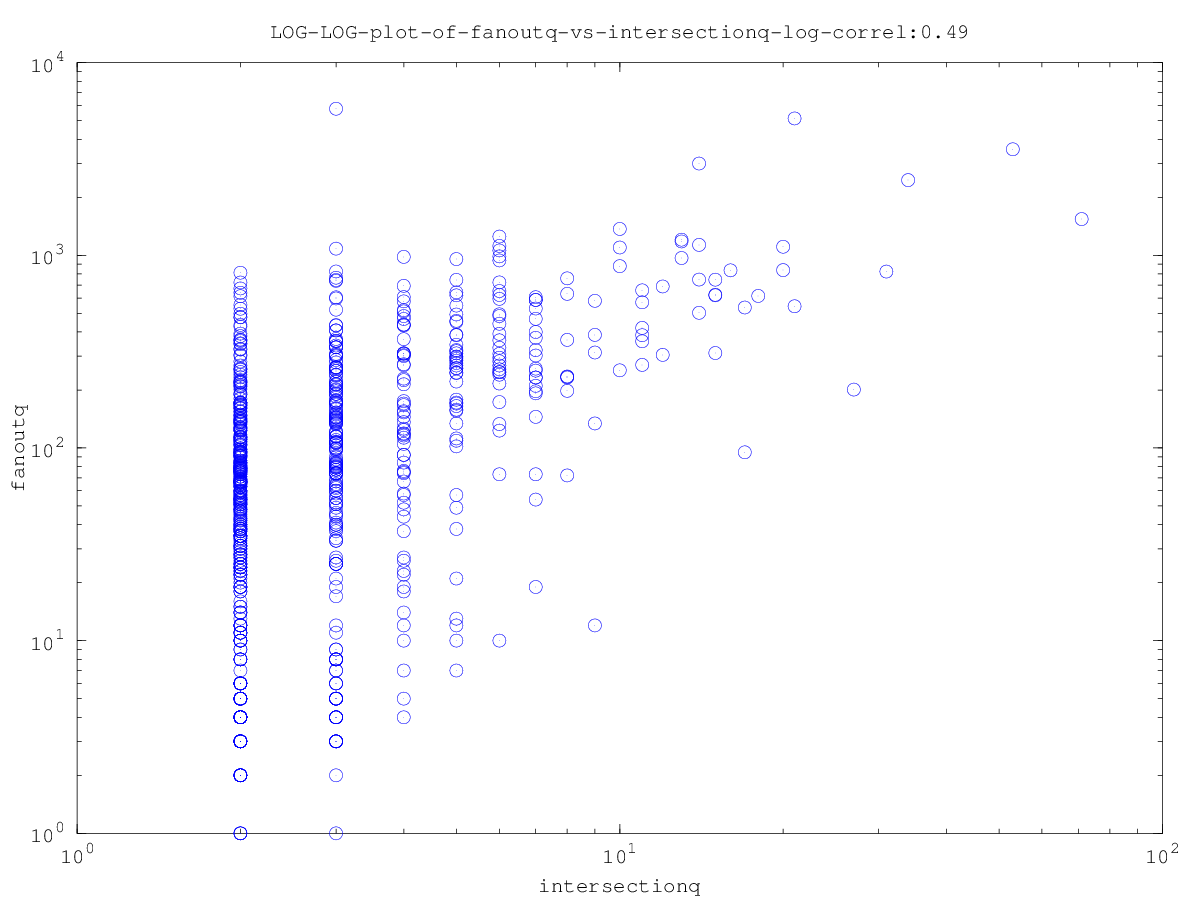
\includegraphics[width=\gridscale]{figures/LOG-LOG-plot-of-fanoutq-vs-intersectionq-log-correl049.png}}\\
 \subfigure{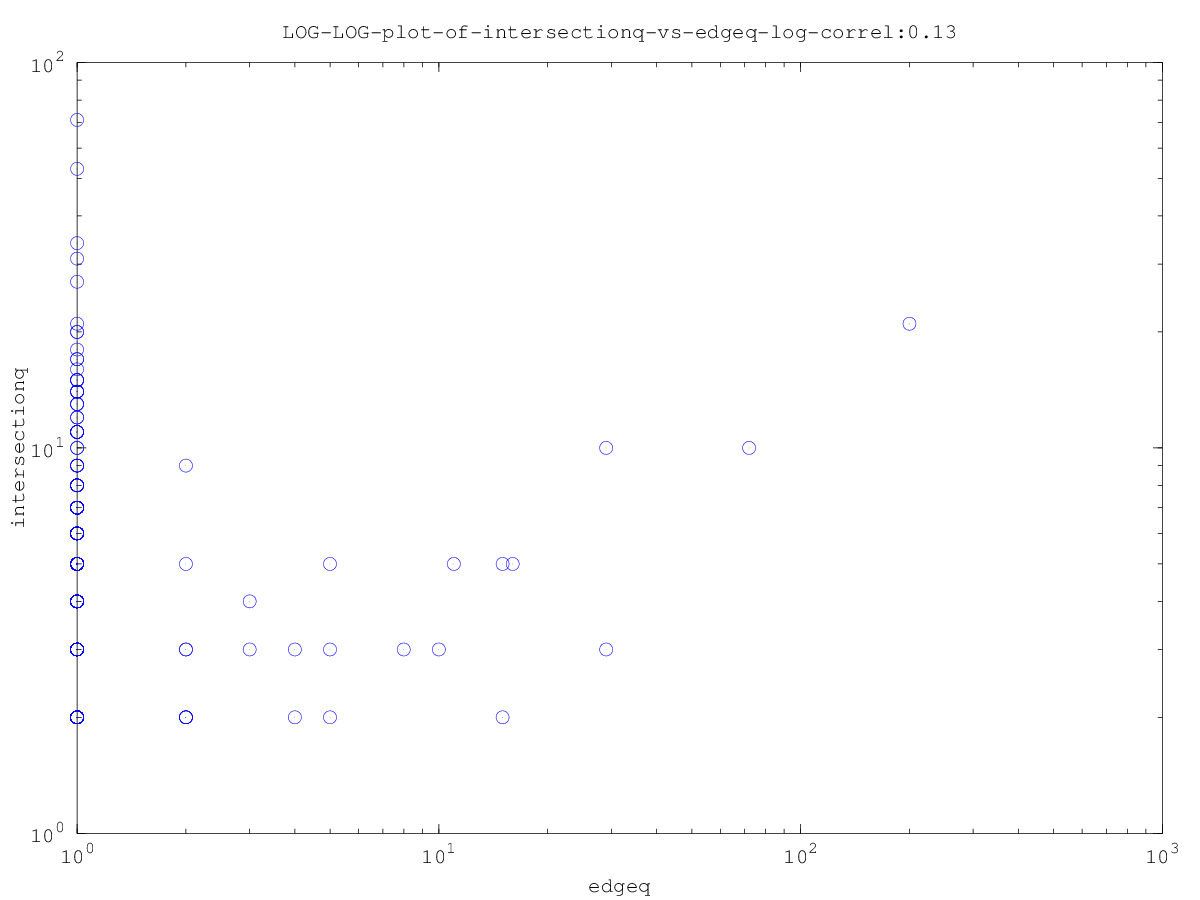
\includegraphics[width=\gridscale]{figures/LOG-LOG-plot-of-intersectionq-vs-edgeq-log-correl013.png}}
\caption{log-log scatterplots of correlations between query types}
\label{fig:querycorr}
\end{figure}

The edge metadata queries happen much less often, so the scatter plot has many points on the zero line (in the log sample). Also, these plots are made on a log-log scale, because they appear somewhat uniform, it implies some users get orders of magnitude more queries than others.   Interestingly, fanout queries and intersection queries are visibly correlated. Edge queries are not not as much. If we remove the nodes that have no edge queries at all, on the other hand, x

\subsection{Data}

As of September 2011 Twitter had an active user population of 100 Million \cite{twitter}.  The total graph stored can only be larger, as it contains all users from all time as well. The total number of edges between these active users is more than an order of magnitude above that, if we assume between 10 and 100 followers per user on average.   For the benchmarks run (described in section \ref{section:benchreal}) I worked with an older snapshot of the graph with 130 million (active and non-active) vertices and an average follower count of 40, for a total of about 5 billion directed edges. For these particular measurements I used a sample of this data set joined with the  sampled query logs of Section \ref{section:workload}.

Like with many other naturally occurring graphs, the degree distribution is similar to a power law: most of the users have relatively small degree (less than 100) but with a still substantial tail of users having larger degrees (the heaviest users have more than 10 million) and the decay behaving like the curve $1/x^2$. The maximum degree was 1 million.  The relation between in-degree (followers) and out-degree (people followed by user) is shown in Figure~\ref{fig:degcorr}.

\begin{figure}
\centering
   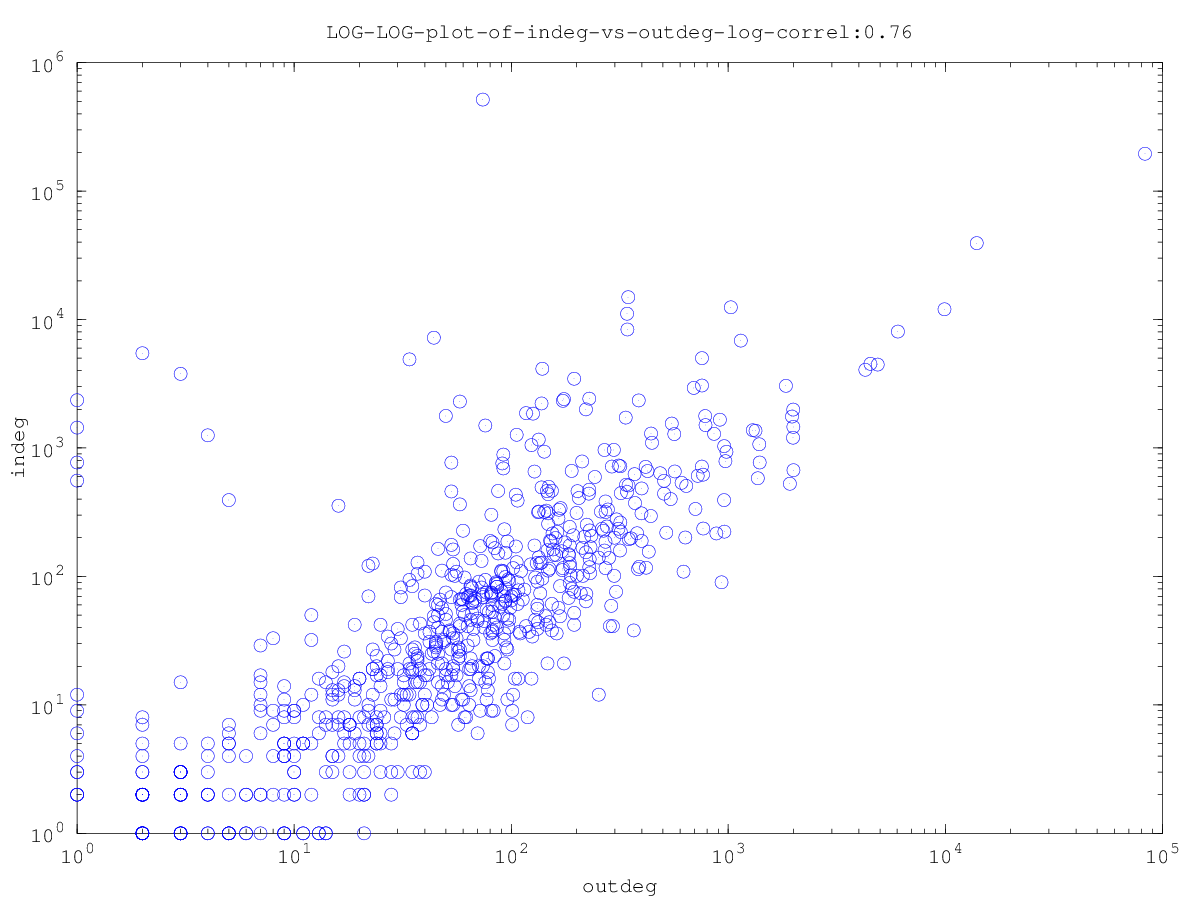
\includegraphics[width=\gridscale]{figures/LOG-LOG-plot-of-indeg-vs-outdeg-log-correl076.png}
   \caption{log-log scatter plot of in-degree vs out-degree}
   \label{fig:degcorr}
\end{figure}


%% %% LOG-LOG-plot-of-fanoutq-vs-edgeq-log-correl019.png          LOG-LOG-plot-of-indeg-vs-outdeg-log-correl076.png
%% %% LOG-LOG-plot-of-fanoutq-vs-intersectionq-log-correl049.png  LOG-LOG-plot-of-intersectionq-vs-edgeq-log-correl013.png
%% %% LOG-LOG-plot-of-indeg-vs-edgeq-log-correl002.png            LOG-LOG-plot-of-outdeg-vs-edgeq-log-correl004.png
%% %% LOG-LOG-plot-of-indeg-vs-fanoutq-log-correl001.png          LOG-LOG-plot-of-outdeg-vs-fanoutq-log-correl006.png
%% %% LOG-LOG-plot-of-outdeg-vs-intersectionq-log-correl009.png

From the figure we can again tell both the out-degree and in-degree distributions (for this small sample) already spans a few orders of magnitude. The in-degree (number of followers) is more spread out than the out-degree (number of people user follows), but they are highly correlated.  One consequence of this is that it may make sense to store the out edges separately from the in edges for heavy weight users at least.

One last measurement of interest is checking for correlations between user degree and workload. In other words, are you queried more if you have more followers or is there no correlation? The possibility of correlation would have implications. If large users were queried less often than smaller users, then optimizing for them is less important. If they are queried very often, relative to smaller users, then they are more significant to the performance metrics. There are arguments why this could happen: perhaps heavy users are much more involved in their accounts, or tweet more often.  Also, nodes with very large degrees imply a write for each of their edges.     By joining the log records from section \ref{section:workload} with the graph snapshot  used, we checked if wthere were any significant trends. The results are shown in Figure~\ref{fig:degworkload}.

\begin{figure}
\centering

  \subfigure{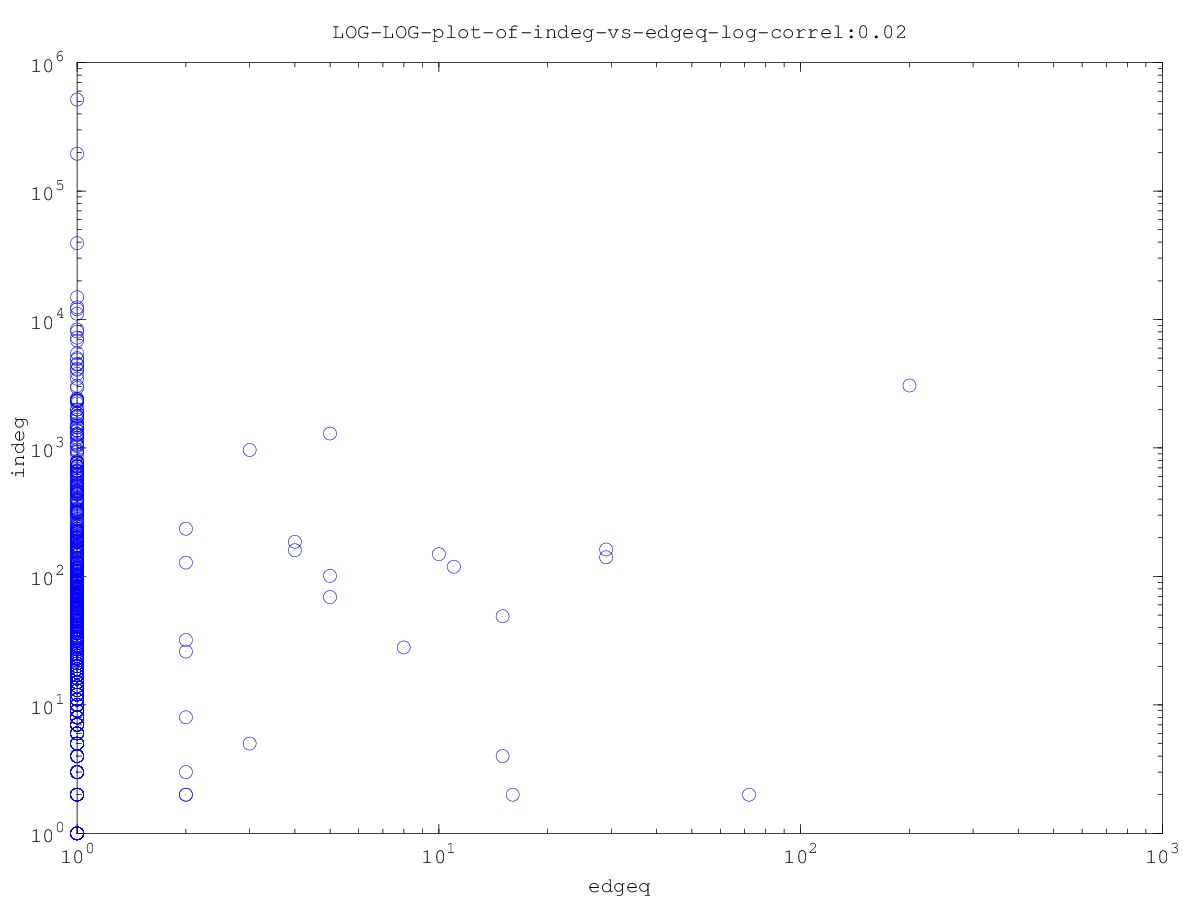
\includegraphics[width=3.5in]{figures/LOG-LOG-plot-of-indeg-vs-edgeq-log-correl002.png}} \\
  \subfigure{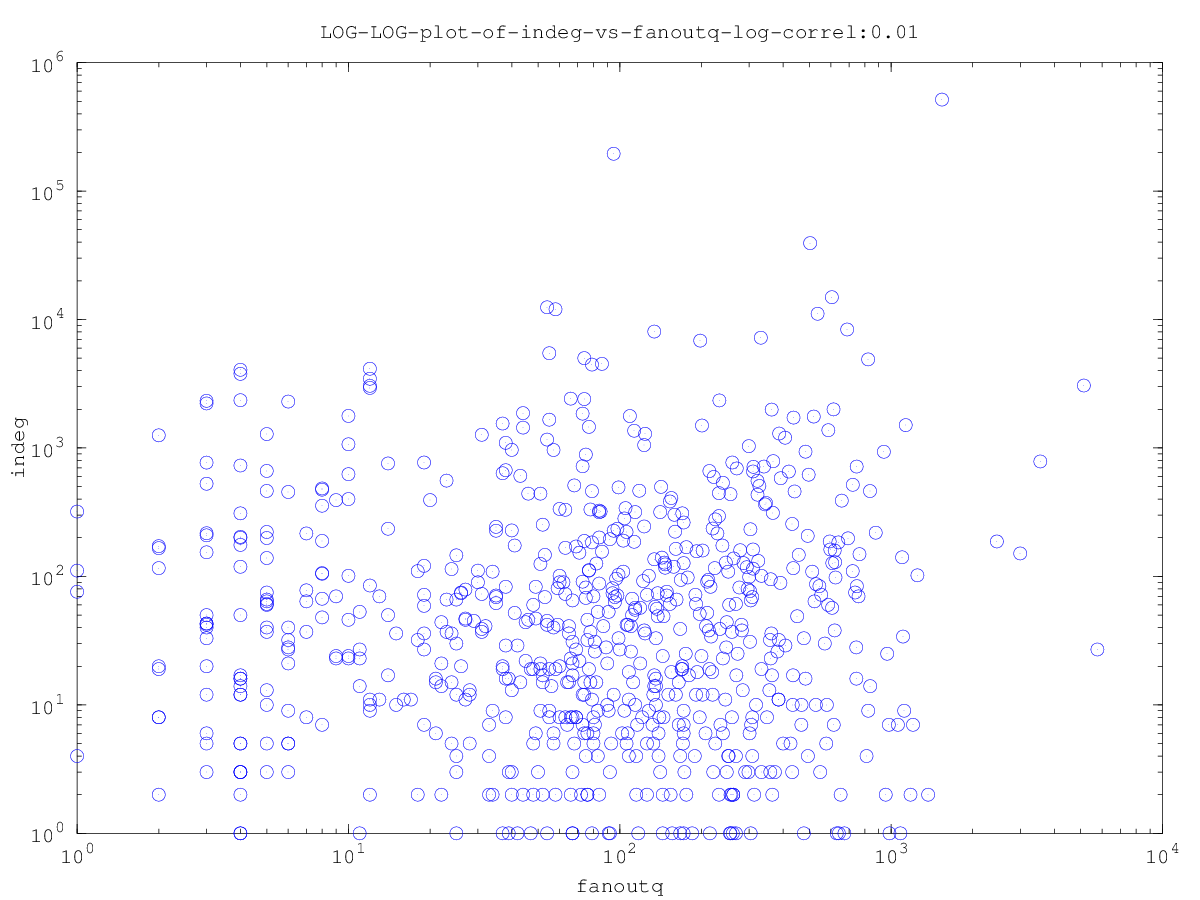
\includegraphics[width=3.5in]{figures/LOG-LOG-plot-of-indeg-vs-fanoutq-log-correl001.png}}\\
  \subfigure{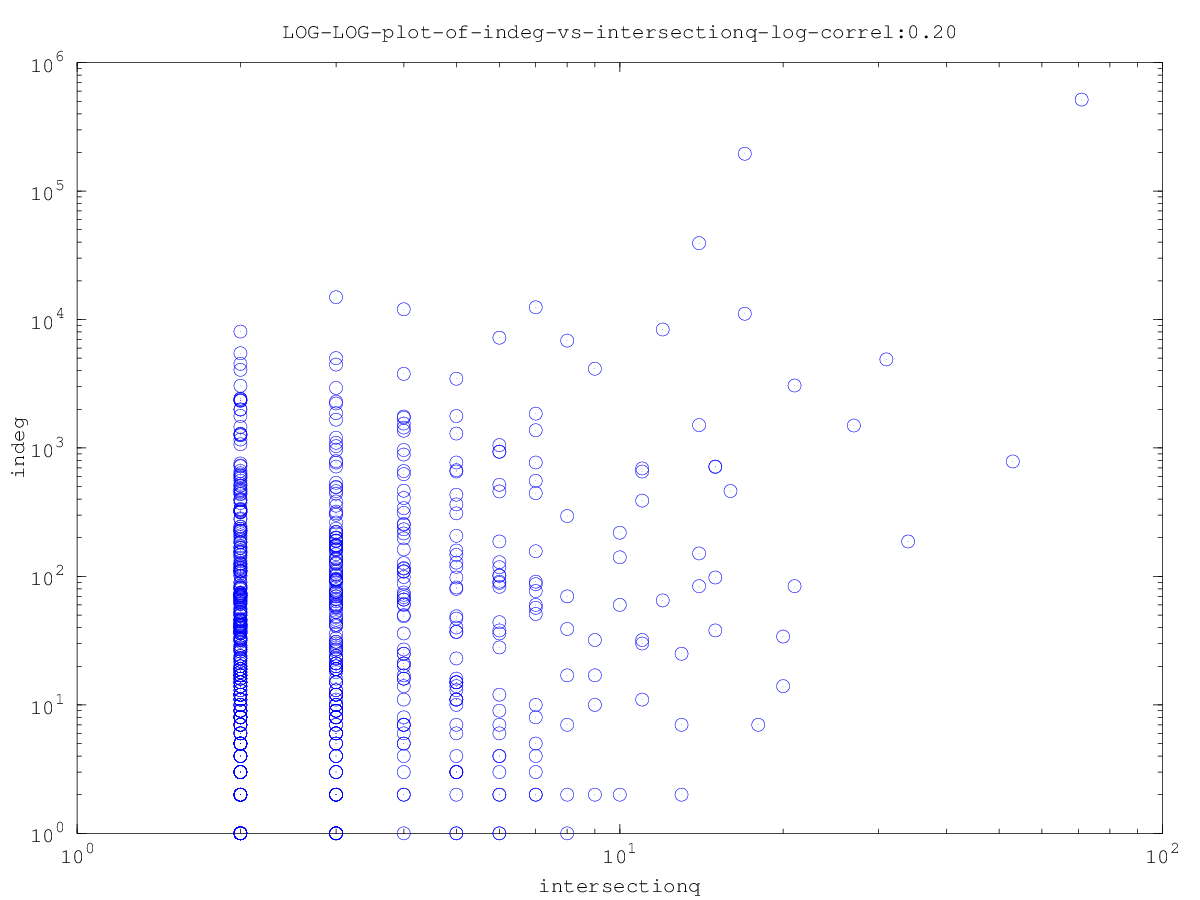
\includegraphics[width=3.5in]{figures/LOG-LOG-plot-of-indeg-vs-intersectionq-log-correl020.png}}\\

\caption{correlations between query popularity and number of followers}
\label{fig:degworkload}

\end{figure}

Edge and fanout queries show little correlaton with in-degree (number of followers), but intersections do show a postive relation.  Out degree (number of people followed by user) relates less strongly with intersection queries.
